% !TEX root = ./cvl.tex
\section{CVL Language}
\label{sec:cvl:language}
The Cartographic Visualization Language (CVL) is a declarative language that can be used to specify an instance of the multi-scale filtering problem. CVL is a rule-based language with a similar goal as other rule-based languages for filtering spatial datasets~\cite{sld,mapnik}, i.e. to control the density of information at each zoom-level. The CVL approach is however markedly different. In the related languages the user must explicitly control the filtering of records at each zoom-level, while also specifying how records are rendered (presentation). First of all, CVL is not concerned with presentation, only filtering. Furthermore, CVL controls filtering in a novel constraint-based way. Instead of having the user explicitly control the filtering of records at each zoom-level, CVL lets the user choose \emph{map constraints} that are instead enforced at all zoom-levels. By making the constraints explicit and the control implicit a very concise formulation is obtained. See Figure~\ref{fig:cvl:example:airports} for an example of this.

CVL is one of the first languages and frameworks to implement the idea of reverse data management~\cite{meliou2011reverse}. In reverse data management, the core idea is that a user states a set of constraints and an objective. These are given together with an input database to an optimization algorithm which computes an output database that is feasible and optimal with regard to the constraints and objective (if a feasible solution exists). This is exactly how CVL works. Furthermore, a feasible solution is guaranteed to exist, as filtering out all records is always a feasible solution.

The CVL language has two statements, the \emph{generalize} statement (see Section~\ref{sec:generalize:statement}) and the \emph{create-constraint} statement (see Section~\ref{sec:create:constraint:statement}). The create constraint statement is used to formulate new map constraints and the generalize statement is used for everything else. 

The CVL language builds on top of SQL and reuses SQL as a language for formulating constraints and record weighting schemes.

\subsection{Generalize statement}
\label{sec:generalize:statement}

The generalize statement is the main statement in CVL. This statement creates a new multi-scale dataset from an input table of geospatial records, subject to user defined constraints. The syntax is shown in Figure~\ref{fig:generalize:syntax}. The statement has several clauses, beginning with the specification of input and output tables. Instead of giving the name of an input table, the user can optionally write a dynamic select statement in SQL of the form \texttt{(SELECT ...) t}. The next clause is the \emph{zoom-levels} clause where the user writes a positive integer, which is the zoom-level  at which the filtering process will begin. The \emph{weigh-by} clause is used to give an arbitrary floating point expression that is evaluated for each row in the input and used as weight for that record. The \emph{subject-to} clause lists the map constraints along with any parameters (as a comma-separated list). The \texttt{AND} keyword is used to separate constraints in the case more than one is used.

For clarity the syntax is shown without two clauses, the \emph{with-id} clause and the \emph{with-geometry} clause, which are used simply to specify the names of the ID and geometry columns in the input table.

\begin{figure}[htbp]
\begin{center}
\begin{lstlisting}
GENERALIZE 
   {input} TO {output}
AT {integer} ZOOM LEVELS
WEIGH BY
  {float expression}
SUBJECT TO 
   {constraint} {float parameters} [AND
   {constraint} {float parameters} [AND
   ...]]
\end{lstlisting}
\caption{Syntax of generalize statement.}
\label{fig:generalize:syntax}
\end{center}
\end{figure}

\begin{figure*}[tb]
  \begin{minipage}{0.329\linewidth}
    \centerline{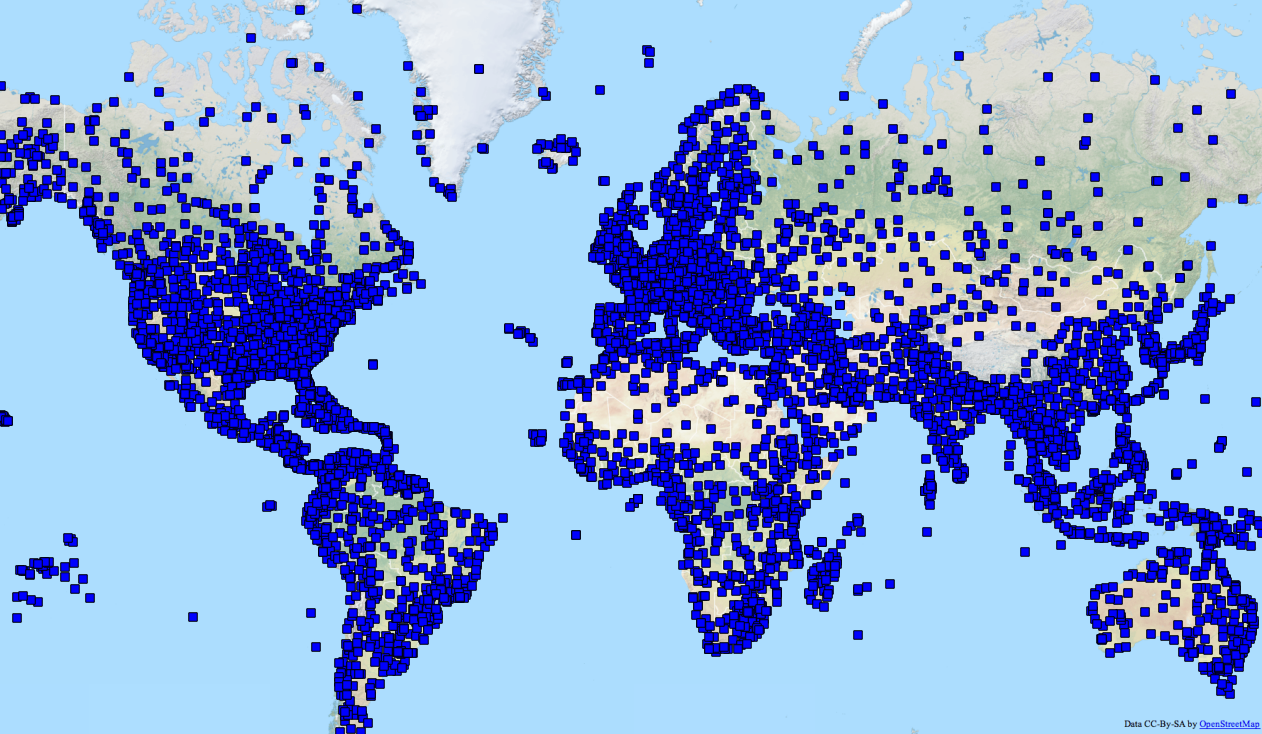
\includegraphics[width=0.95\linewidth]{./figs/airports.png}}
    \centerline{(a) Full Openflights Airport dataset}
  \end{minipage} \hfill
  \begin{minipage}{0.329\linewidth}
    \centerline{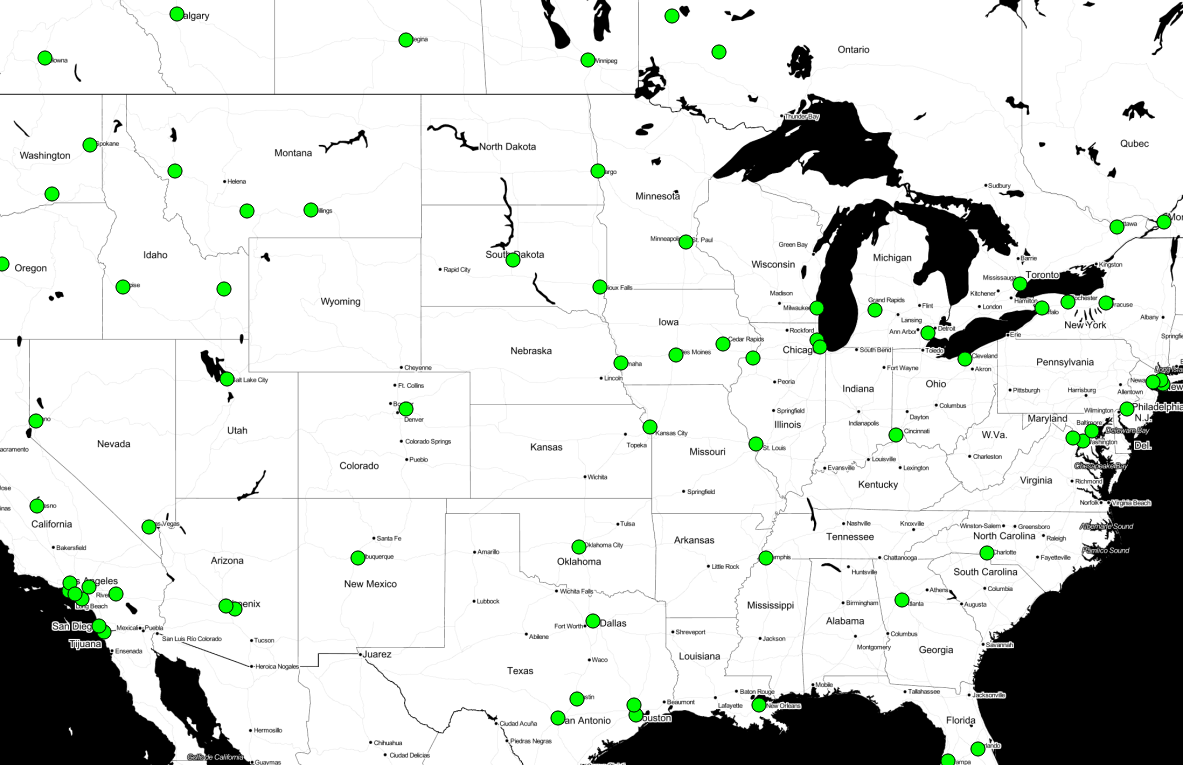
\includegraphics[width=0.95\linewidth]{./figs/airports_z4.png}}
    \centerline{(b) Airports on zoom-level 5}
  \end{minipage} \hfill
  \begin{minipage}{0.329\linewidth}
    \centerline{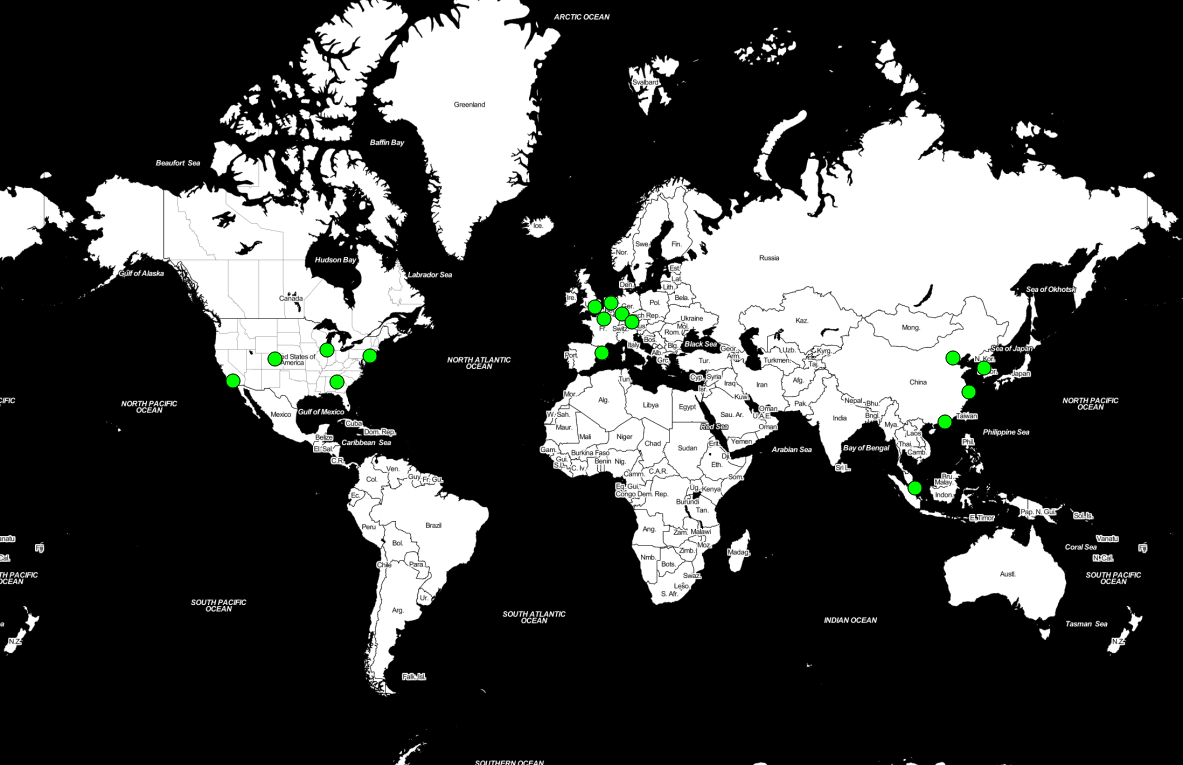
\includegraphics[width=0.95\linewidth]{./figs/airports_z0.png}}
    \centerline{(c) Airports on the top-most zoom-level.}
  \end{minipage}
  \vspace{-0ex}
  \caption{Airport map (7K points) before (a) and after (b, c) running CVL. The output corresponds to the CVL statement in Figure~\ref{fig:cvl:example:airports}.}
  \label{fig:graphical:output:airport}
  \vspace{-2ex}
\end{figure*}

An example of generalizing a dataset using the generalize statement is shown in Figure~\ref{fig:cvl:example:airports}. In this example a dataset containing point records representing the location of airports world-wide is generalized. The records are weighted by using the name of a column containing the number of routes departing from each airport (CVL automatically handles the cast from integer to floating point). The intuition is that airports with more departures are more important. The single constraint that is enforced is the visibility constraint, with a parameter of $K=16$. Recall that the visibility constraint says that each tile can contain at most $K$ records.

\begin{figure}[htbp]
\begin{center}
\begin{lstlisting}
GENERALIZE 
   airports TO airports2
AT 18 ZOOM LEVELS
WEIGH BY
  num_departures
SUBJECT TO 
   visibility 16 
\end{lstlisting}
\caption{Generalization of an airports dataset. The airports are weighting by number of departures. See Figure~\ref{fig:graphical:output:airport} for a vizualization of the result.}
\label{fig:cvl:example:airports}
\end{center}
\end{figure}

The resulting map is shown in Figure~\ref{fig:graphical:output:airport} and has at most $16$ airports on each tile. For the top zoom-level these are the 16 biggest airports in the world. The CVL framework automatically gives priority to the airports with the highest weight. How this is done is explained in sections~\ref{sec:optimizationmodel} and~\ref{sec:algorithms}.

\subsection{Create constraint statement}
\label{sec:create:constraint:statement}

% change text
Map constraints are defined using the create-constraint statement.  The basic syntax of the statement is shown in Figure~\ref{fig:create:constraint:syntax}. The body of the statement is a SQL select statement that selects tuples $\langle cid, rid\rangle$ representing conflicts that are found at a given zoom-level in the map. See Section~\ref{sec:conflicts} for the semantics of the tuples.

The \emph{resolve-if-delete} clause is used to compute the integer number of records that must be deleted in order to resolve the conflict with a given $cid$. 
%For the proximity constraints this number is always 1, but for other constraints this may vary.

\begin{figure}[htbp]
\begin{center}
\begin{lstlisting}
CREATE CONSTRAINT C1
AS NOT EXISTS
  {SQL select statement}
  
RESOLVE cid IF DELETE (
  {integer expression}
)
\end{lstlisting}
\caption{Syntax of create constraint statement}
\label{fig:create:constraint:syntax}
\end{center}
\end{figure}

Using this syntax, the definition of the proximity constraint is given in Figure~\ref{fig:proximity:definition}. The body of the constraint is a distance self join using a distance function \texttt{ST\_Distance} provided by a spatial extension to SQL. This join finds all pairs of records that are too close, e.g.\ less than $10$ pixels apart. For each conflict, the select statement outputs two tuples and exactly once for each conflict. The resolve-if-delete clause is simply the constant $1$, because that is how many records must be deleted to resolve a proximity conflict.

\begin{figure}[htbp]
\begin{center}
\begin{lstlisting}
CREATE CONSTRAINT Proximity
AS NOT EXISTS (
  SELECT 
    l.{rid} || r.{rid} AS cid,
    Unnest(array[l.{rid}, r.{rid}]) AS rid
  FROM
    {level_view} l
  JOIN
    {level_view} r
  ON
    l.{rid} < r.{rid}
  AND
    l.{geom} && ST_Expand(r.{geom}, 
      CVL_Resolution({z}, 256) * 
        {parameter_1})
  AND
    ST_Distance(l.{geom}, r.{geom}) <
      CVL_Resolution({z}, 256) * {parameter_1}
)

RESOLVE cid IF DELETE (
  1
)
\end{lstlisting}
\caption{Definition of the proximity constraint.}
\label{fig:proximity:definition}
\end{center}
\end{figure}

In Figure~\ref{fig:proximity:definition} some names are enclosed in curly braces like \texttt{\{rid\}}. These are variables which are bound at runtime by the CVL framework and are intended for making the definition of constraints simpler. The variables \texttt{\{rid\}} and \texttt{\{geom\}} are bound to the column names containing the ID and geometry of the records. The \texttt{\{level\_view\}} is bound to a view that contains all records that are visible at the current level, i.e., the records that have not been filtered out at a higher zoom-level. The function \texttt{CVL\_Resolution(\{z\}, 256)} is one of the utility functions defined by the CVL runtime, also with the purpose of making the definition of constraints simpler. This function returns the resolution (meter/pixel) at zoom-level \texttt{\{z\}}, where \texttt{\{z\}} is a variable bound to the currently evaluated zoom-level. The variable \texttt{\{parameter\_1\}} is the constraint parameter, e.g. $10$ pixels.

\vspace{5em}

Figure~\ref{fig:visibility:definition} shows how the visibility constraint may be defined using CVL. The CVL definition uses an extension of the basic create-constraint syntax, namely the \emph{setup} and \emph{tear down} clauses. 
%which will be covered again in Section~\ref{sec:implementation:extensions}. 
The purpose of these clauses is to enable arbitrary SQL statements to be run before and after the constraint body is evaluated at each zoom-level. During the setup phase we create an auxiliary table called \texttt{busted\_tiles} which contains tuples $\langle tile\_id, rid \rangle$ identifying tiles that are intersected by more than $K$ records, and the ID of those records. The body of the constraint simply iterates over the auxiliary table, using the \texttt{tile\_id} column as the conflict ID.

The user does not need to know how the conflicts are handled, because all conflicts are automatically resolved by the CVL framework using one of the algorithms presented in Section~\ref{sec:algorithms}.

%In this example, calls are made to other CVL runtime functions, namely \texttt{CVL\_WebMercatorCells} and \texttt{CVL\_PointHash}. These functions returns a set of points corresponding to the centroids of intersected tiles (given a geometry) and a unique identifier for points, respectively. The unique identifier for points is based on the well-known GeoHash algorithm.

\begin{figure}[htbp]
\begin{center}
\begin{lstlisting}
CREATE CONSTRAINT Visibility
AS NOT EXISTS (
    SELECT
        busted_tiles.cid,
        busted_tiles.rid
    FROM
        busted_tiles
)

RESOLVE cid IF DELETE (
  SELECT count(*) - {parameter_1}
  FROM   busted_tiles bt
  WHERE  bt.cid = cid
)

WITH SETUP (
    CREATE TEMPORARY TABLE busted_tiles AS (
        SELECT
            t.cid,
            Unnest(array_agg(t.cvl_id)) AS rid
        FROM
        (
        SELECT
            CVL_PointHash(CVL_WebMercatorCells({geometry}, {z})) AS cid,
            {rid}
        FROM
            {level_view}
        ) t
        GROUP BY t.cid
        HAVING count(*) > {parameter_1}
    );
    CREATE INDEX busted_tiles_id_idx ON busted_tiles (cid);
)

WITH TEARDOWN (
  DROP TABLE busted_tiles;
)
\end{lstlisting}
\caption{Definition of the visibility constraint.}
\label{fig:visibility:definition}
\end{center}
\end{figure}

% give the variables by example, and explain together with the example, instead of listing everything up front.

%\marcos{These could be introduced by need along with the examples integrated into the sections above.}
